\documentclass[main.tex]{subfiles}
\begin{document}
\onlyinsubfile{\mainmatter{}}

\chapter{Glyco: A Nanopass Compiler for CHERI-RISC-V}
Glyco\footnote{From the Greek term $\gamma\lambda\upsilon\kappa{}o$ meaning \enquote{sweet}, alluding to the taste of a wild cherry.} is a compiler targeting the CHERI-RISC-V architecture, producing software running on CheriBSD systems and on a Sail-based emulator of the CHERI-RISC-V ISA.

We begin by giving a concise description of the nanopass compiler design, which is used for Glyco. We then describe the design \& implementation of the base compiler, a compiler that emits CHERI-RISC-V instructions but has almost no additional features taking advantage of the capability machine proper. We do so using a few example programs, working our way from the high-end language to the machine language. A full language reference of the final compiler can be found in \cref{ch:grammar}.

Later chapters discuss extensions and changes to this first version of the compiler.

\section{Background: Nanopass Compilers}
Glyco is built following a \emph{nanopass} compiler design, described in the context of compiler education by several authors such as \cite{educomp} and in the context of commercial compiler development by authors such as \cite{commcomp}. A nanopass compiler consists of numerous small passes, so-called \emph{\glspl{nanopass}}, which translate one \emph{\il{}} to another. Source code is parsed into the compiler’s first \il{}, which is then translated via \glspl{nanopass} through different \ils{}, ending up in the compiler's final \il{}. This final \il{} contains a string representation of the assembly code that is fed to the Clang compiler from the LLVM compiler toolchain for building \& linking an executable ELF file. This last step is unrelated to the research problem, hence this dependency on LLVM.

The nanopass design allows the compiler engineer to design and implement their compiler \emph{by iterated abstraction}. A simplified description follows. The engineer first chooses a target language (usually a machine language such as x86-64 or indeed CHERI-RISC-V) and determines an abstraction over it. The engineer then defines an \il{} that implements that abstraction as well as a \gls{nanopass} which transforms programs written in the new \il{} to the target language. The compiler engineer then repeats this process, this time abstracting over the \il{} with a new \il{} and \gls{nanopass}. This process goes on until a level of abstraction has been reached that can either be directly used as a source language (by human users), or be easily produced by parser actions.

An important benefit of the nanopass approach is each new iteration begins and ends with a working compiler. After each iteration, users can start writing and compiling programs in the new \il{} and unit tests can be written that ensure that the new \gls{nanopass} produces the expected transformations. For experimental architectures such as CHERI-RISC-V, this also means that designers can experiment more quickly with new ideas, something that may be harder to do on a full-fledged production compiler such as Clang.

Glyco defines 20 \gs{il}, with a general approach adapted from the student compiler by \cite{compcourse}. Each language is named after the new abstraction or feature it brings compared to the \g{lowerlang}. We discuss the \gs{il} in reverse chronological order (from high-level to low-level languages) as opposed to the order in which the \gs{il} were defined (from low-level to high-level languages). This allows us to explain the compiler pipeline using example programs, showing how they are manipulated by the compiler's \gs{nanopass}.

\section{An Expression Language}
The highest \il{} in the first version of Glyco is called \textbf{EX} (Expressions), a language with basic support for arithmetic operations, functions, conditionals (\texttt{if}-\texttt{then}-\texttt{else}), definitions (\texttt{let}-bindings), vectors (fixed-size arrays), and records (collections of key-value pairs).

The following EX program computes the 30th number in the Fibonacci sequence starting with 0 and 1:
\lstinputlisting{Programs/fib.ex}

This program defines a function \texttt{fib} with three signed 32-bit integer parameters \texttt{prev}, \texttt{curr}, and \texttt{iter} and which returns a signed 32-bit integer. The function recursively adds the \enquote{previous} and \enquote{current} sums until the number of iterations drops to 0, then returns the \enquote{current} sum. The program itself is defined as the result of \texttt{fib} where \texttt{prev} is 0, \texttt{curr} is 1, and \texttt{iter} is 30.

EX is an \emph{intermediate} language and not necessarily a \emph{user-friendly} language; it is instead quite explicit and contains little syntactical sugar. For example, a value representing the constant 30 is written as \texttt{constant(30)}, the value of a variable or parameter named \texttt{iter} is written as \texttt{named(iter)}, and the predicate $ \textit{iter} \le 0 $ is written as \texttt{relation(named(iter), le, constant(0))}. A significant benefit is that the structure is easy to manipulate as the code goes through the compiler's \gs{nanopass}. One can, however, define a more user-friendly language and write a parser that emits EX.

\paragraph{From EX (Expressions) to LS} LS does not support subexpressions so the \g{nanopass} to LS binds all subexpressions to names (temporaries) and uses those names in place of the subexpressions. For instance, the EX value
\begin{lstlisting}
	evaluate(function(fib), ... binary(named(prev), add, named(curr)) ...)
\end{lstlisting}
is transformed into the equivalent LS value
\begin{lstlisting}
	let(
		(arg0, ...) (arg1, let(
			(ex.lhs, source(named(prev))) (ex.rhs, source(named(curr))),
			in: binary(named(ex.lhs), add, named(ex.rhs))
		)) (arg2, ...),
		in: evaluate(fib, named(arg0) named(arg1) named(arg2))
	)
\end{lstlisting}

Some transformations are not strictly necessary, e.g., binding \texttt{named(prev)} to \texttt{ex.lhs} instead of using \texttt{named(prev)} directly. They do not however incur any additional overhead in the final executable: a \g{nanopass} further down the compiler pipeline cleans up these redundant temporaries.

\paragraph{From LS (Lexical Scopes) to DF} DF does not support shadowing; all \texttt{let} bindings are in a single namespace. The \g{nanopass} from LS to DF implements shadowing by renaming symbols such that each definition uses a globally unique symbol.

\paragraph{From DF (Definitions) to CV} CV does not support \texttt{let} bindings, i.e., definitions. The \g{nanopass} implements them in CV using \texttt{do} values, i.e., computed values, which are values on which a computation can be attached. For example, the DF value
\begin{lstlisting}
	let((answer, source(constant(42))), in: source(location(answer)))
\end{lstlisting}
is \lowered{} to the CV value
\begin{lstlisting}
	do(set(answer, to: source(constant(42))), then: source(location(answer)))
\end{lstlisting}

\paragraph{From CV (Computed Values) to CA} CA does not support \texttt{do} values, but does support \texttt{do} effects, which are sequences of effects. The \g{nanopass} implements \texttt{do} values by extracting their effects into \texttt{do} effects and ending with an additional \texttt{set} effect that moves the result to the intended destination. That is, a CV \texttt{set} effect
\begin{lstlisting}
	set(result, to:
		do(
			/* effects */,
			then: /* result */
		)
	)
\end{lstlisting}
is transformed to a CA \texttt{do} effect
\begin{lstlisting}
	do(
		/* effects */
		set(result, to: /* result */)
	)
\end{lstlisting}

\paragraph{From CA (Canonical Assignments) to CC} The final purely structural transformation lowers \texttt{set} effects in CA using equivalent effects in CC, only keeping the \texttt{set} effects with a constant or location source. For example, the CA program
\lstinputlisting{Programs/values.ca}
is lowered to the CC program
\lstinputlisting{Programs/values.cc}

\section{A Conventional Calling Convention}
A \g{cc} is a set of rules imposed by the operating system, instruction set architecture, and/or programming language that specify how procedures are called. A low-level \g{cc} often specifies
\begin{itemize}[noitemsep]
	\item where parameters and result values are placed (in dedicated registers, in a particular order on the call stack, or a combination of both);
	\item how large values are passed to the callee or caller (over multiple registers, on the call stack, or in heap memory), if supported;
	\item the state of the call stack and some registers (like the register keeping the frame pointer) when a procedure starts executing and when it returns to the caller;
	\item which registers a procedure can use freely but for which it cannot assume that their contents will be preserved across a procedure call (\textbf{\gs{cersaved}}); and
	\item which registers a procedure can only use after saving their previous contents and if they're restored after use (\textbf{\gs{ceesaved}}).
\end{itemize}

The \g{cc} used in the base version of Glyco is called \textbf{\g{gccc}} and mimics a traditional \g{cc} that would be used for programs written in C, with some parts specified by \cite[chapter~25]{riscv}.

\paragraph{Call stack} The call stack is a region of memory on which information about procedure calls is stored, such as local state and return addresses. The stack grows downward, i.e., from high to low addresses. The \texttt{csp} register contains the \textbf{\g{stackcap}}, a capability that points to the location of the last pushed datum, i.e., the top of the stack, and gives read-write authority over the stack memory. The \g{stackcap}'s address decreases whenever data are pushed to the call stack and increases whenever data are popped from the stack.

\paragraph{Call frames} A call frame (also known as a \emph{stack frame}) is a region of memory on the call stack that belongs to a procedure call and on which the procedure can store its local state. The \texttt{cfp} register contains the \textbf{\g{framecap}}, a capability derived from the \g{stackcap} that points to the base of the call frame. The procedure places local state and expects parameters in locations that are fixed distances removed from this base.

Before accessing its call frame, a procedure pushes a call frame of the desired size to the call stack in three steps. The procedure first pushes the (caller's) \g{framecap} to the call stack, then updates the \g{framecap} to point to this capability, and finally allocates room for its local state by moving the \g{stackcap} so that it points to the new call frame's last datum.

A procedure pops its call frame when it is done using it, e.g., when returning to its caller. It does so by popping all data stored in the call frame and restoring the previous \g{framecap}.

\paragraph{Parameters} Arguments to parameters are passed to the callee via dedicated argument registers first. When the set of argument registers is exhausted, any remaining arguments are pushed (in order) to the stack where they become part of the caller's call frame for the duration of the call.\footnote{This is the only part of another procedure's call frame that a callee is allowed to access directly.} Since these \emph{frame-resident} arguments reside at higher addresses than the callee's \g{framecap}, the callee can access these arguments using positive offsets of the \g{framecap}.

The set of argument parameters in Glyco is customisable via a command-line option. The default set is \texttt{a0}, \texttt{a1}, \texttt{a2}, \texttt{a3}, \texttt{a4}, \texttt{a5}, \texttt{a6}, and \texttt{a7}.

All of Glyco's supported data types in Glyco fit in a register. Vectors and records are returned by reference as capabilities.

\paragraph{Results} A procedure can return a single value via \texttt{a0}. Vectors and records are passed by reference as capabilities.

\paragraph{Available registers} The set of \gs{cersaved} and \gs{ceesaved} registers is customisable via command-line options. The default \gs{cersaved} are \texttt{s1}, \texttt{s2}, \texttt{s3}, \texttt{s4}, \texttt{s5}, \texttt{s6}, \texttt{s7}, \texttt{s8}, \texttt{s9}, \texttt{s10}, and \texttt{s11}; the default \gs{ceesaved} are the remaining 9 registers available in CC.

\paragraph{Local state} A procedure call's local state comprises saved register data (cf. supra), data for which no register is available, and stack-allocated buffers. These are reside at lower addresses than the call's \g{framecap}; the procedure can therefore access them using negative offsets of the \g{framecap}.

\paragraph{Return address} The caller provides a return address capability in the \texttt{cra} register.\footnote{\texttt{cra} is a \g{ceesaved}, so if the callee needs to call another procedure, it will need to save the contents of \texttt{cra} before overwriting the register, except in the special case of a tail-call.} The callee can return control to the callee by jumping to this return capability.

\Cref{fig:gcccstack} shows a simple two-frame call stack example with zero registers available for arguments and local variables, to force Glyco to store them in call frames.

\begin{figure}
	\begin{center}
		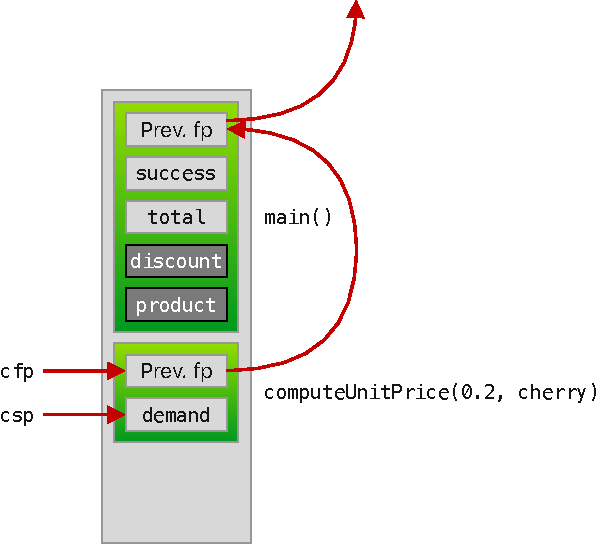
\includegraphics{Images/GCCC Stack.pdf}
	\end{center}
	\caption{A call stack containing two call frames in a configuration of GCCC where no registers are available for storing parameters and local variables. The first call frame belongs to the initial procedure \texttt{main} which is called by the runtime, a dynamic linker, or the operating system and takes no parameters. Its call frame contains a \emph{previous frame pointer} capability that points to an unspecified location (possibly \texttt{null}) as well as two local variables \texttt{discount} and \texttt{price}. \texttt{main} invokes the 2-parameter \texttt{computeUnitPrice} procedure, binding the value \texttt{0.2} to the \texttt{discount} parameter and \texttt{cherry} to the \texttt{product} parameter. The latter procedure's call frame contains a \emph{previous frame pointer} capability that points to the location of the \emph{previous frame pointer} capability in the previous call frame, as well as a local variable \texttt{demand}. This call frame is at the top of the stack and so the \texttt{cfp} register's capability points to the \emph{previous frame pointer} capability in \texttt{computeUnitPrice}'s call frame. The \texttt{csp} register's capability always points to the last datum pushed on the stack, which is \texttt{demand} in this example. Note that the stack grows downward.}
	\label{fig:gcccstack}
\end{figure}

\hspace{0pt} \\
CC (Calling Convention) introduces procedures with parameters and results. It is \lowered{} to its \g{lowerlang} SV by imposing the \g{cc} described above. For example, the CC program
\lstinputlisting{Programs/42.cc}
is lowered to the following SV program:
\lstinputlisting{Programs/42.sv}

The CC to SV \g{nanopass} implements \g{cersaved} preservation by binding the registers' contents to temporary names before the call, and restores those registers' contents after the call. % TODO: Remove those dead moves so that we can claim here that ALA will clean those redundant sets.

\section{Structured Values}
The next \g{il}, \textbf{SV} (Structured Values) provides a structured abstraction over unstructured buffers in the form of \textbf{vectors} and \textbf{records}. A vector in SV is a homogeneous\footnote{All elements are of the same data type.} fixed-size\footnote{The number of elements is determined at creation and can only be changed by creating a new vector of the desired size and moving all elements to it.} array and is represented with a capability that points to the vector's first element, similarly to an array in the C programming language. A record is a heterogeneous\footnote{Values are not necessarily of the same data type.} key-value map with fixed keys and is similar to a C \texttt{struct}. However, unlike C \texttt{struct}s and like SV vectors, a record is represented with a capability that points to the record's first value. Vectors and records in SV are always passed by reference and never implicitly copied. Vector and record capabilities are automatically bounded to the region of memory they occupy; indexing a vector with an index that exceeds the vector's length causes a machine trap.\footnote{Due to CHERI-RISC-V bounds compression, a buffer capability may grant a larger region of memory than requested during allocation, meaning that some \enquote{out of bounds} indices near the end index may actually be valid and not cause a trap. Glyco compensates for this by allocating the extra memory granted by the buffer capability.}

Structured values are implemented in the \g{lowerlang} ID by translating effects dealing with them into effects dealing with unstructured data buffers. For example, the SV program
\lstinputlisting{Programs/sequences.sv}
is \lowered{} to the following ID program:
\lstinputlisting{Programs/sequences.id}
% TODO: Highlight corresponding parts

The results of the \texttt{sll} (logical left shift) operations in this program are statically computed as part of an optimisation pass in a lower \g{il}.

\section{Abstract Locations}
All programs until now have been able to bind values to names in one form or another, be it \texttt{let} bindings with shadowing or globally scoped names or arbitrarily named locations. These names refer to physical locations where data can be stored, but since the programmer does not specify the names themselves are \textbf{abstract locations}, locations that the compiler is to associate with a \textbf{physical location}.

Since registers are orders of magnitude faster to access than locations in RAM, the compiler attempts to assign as many abstract locations as it can to registers in a process called \textbf{register allocation}. Since the number of registers is limited, the compiler may need to \emph{spill} abstract locations to locations on the call frame. Glyco employs several heuristics to minimise the runtime cost by spilling abstract locations that it thinks will be accessed the least.

% TODO

\section{Structured Jumps \& Branches}
% TODO

\section{Basic Abstractions over Assembly}
% TODO

\biblio{}
\onlyinsubfile{\glsaddall\printglossaries}
\end{document}
